% Author Name: José Areia 
% Author Contact: jose.apareia@gmail.com
% Version: 1.0.3 - 18/04/2025
% Public Repository: https://github.com/joseareia/nob-article

% Packages & Document Configurations
\documentclass[twocolumn]{NobArticle}
\runninghead{Parking Mesh: RL-Based Urban Parking Network}
\footertext{\textit{IE University} (May 2025)}
\usepackage{caption}
\captionsetup{justification=centering, singlelinecheck=false}
\usepackage{float}
\usepackage{tabularx}
\usepackage{booktabs}
\usepackage{placeins}
\usepackage{ragged2e}   
\usepackage{flafter}

% Title
\title{Parking Mesh: A Reinforcement Learning-Driven Vehicle Network for Real-Time Urban and Decentralized Parking Optimization}

% Authors
\author{
    Paul Ruiz Alliata, 
    Daniel Kumlin,
    Alberto Puliga,
    Daniel Alves Rosel, 
    and Tomás Mesalles Mejía
}

% Affiliations
\date{
    IE University School of Science and Technology
}

% Executive Summary
\renewcommand{\maketitlehookd}{%
\vspace{2em}
\noindent\textbf{\Large Executive Summary}\par
\vspace{0.5em}
\noindent
Parking Mesh transforms every parked vehicle into a node within a city-wide mesh network that senses adjacent parking gaps and relays real-time vacancy data. By equipping cars with four ultra-low-power proximity sensors and a Bluetooth-mesh microcontroller, we create a self-organizing network that dynamically feeds into a live parking map, minimizing search traffic, cutting emissions, and saving drivers valuable time.    
\medskip

\small{\textbf{Index Terms:} Smart Parking, Multi-Agent Systems, Reinforcement Learning, Bluetooth Mesh, Graph Neural Networks, Urban Mobility, Real-Time Sensing, Decentralised Infrastructure}

}


\begin{document}

\small
\maketitle

\section{Business Introduction}
\subsection{Problem}
Urban drivers waste \$345 billion annually circling for parking spaces in urban environments \footcite{CHEM}. This inefficiency stems from the fundamental challenge of information asymmetry - drivers enter parking areas with no reliable way to determine where available spaces exist. They circle blocks repeatedly, wasting time, fuel, and adding to urban congestion and pollution.
\subsection{Solution}
Our innovation transforms every equipped vehicle into an active node within a city-wide mesh network. By attaching a simple, ultra-low-cost retrofit device to vehicles, we enable them to sense adjacent parking vacancies and relay this information in real-time. This creates a self-organizing network where parked cars themselves become the infrastructure that solves the parking problem. Then, for the drivers to see the available vacancy they will see it with an app their carplay display that will show in real time where they need to go for their parking spot.

When a driver approaches their destination, our system provides instant guidance to the nearest available parking space based on live data from the surrounding vehicle network. No more circling, no more guessing, and no wasted time or fuel.
\subsection{Value Proposition}
Our parking solution fundamentally re-imagines the approach to solving urban parking challenges by transforming every equipped vehicle into a node in a decentralized sensing network. Unlike traditional fixed-infrastructure systems that require massive upfront capital, lengthy municipal approvals, and remain vulnerable to system-wide failures, our ultra-low-cost vehicle retrofit creates an organic mesh network that grows stronger with each adoption.
While existing solutions rely on expensive sensors embedded in streets or garages, our approach leverages the very vehicles causing congestion to become the solution—providing real-time, accurate parking availability data precisely where it's needed most, scaling automatically in high-demand areas, and delivering immediate ROI through saved time and fuel while reducing emissions. By eliminating the need for fixed infrastructure and municipal coordination, we've created a solution that can be implemented immediately, at a fraction of the cost, while providing superior reliability through its distributed architecture.

Parking Mesh is positioned to address a \$5.8 billion smart-parking market (2023) \footcite{MarketResearchFuture2032}, projected to grow to \$14.1 billion by 2033 \footcite{MarketResearchFuture2032}, while also aligning with the \$5.6 billion parking-management sector \footcite{StraitsResearch2033} and tapping into the \$7.7 billion automotive sensor-aftermarket\footcite{GrandViewResearch2030} opportunity.
 
\subsection{Target Persona}
Our solution targets urban drivers who experience significant frustration with daily parking. These individuals value their time highly and feel stressed by the unpredictability of finding parking in congested areas. They typically commute to busy districts where parking is limited and spend 5-15 minutes daily searching for spaces, creating both financial costs from wasted fuel and emotional strain from the anxiety about being late.

Their primary pain points include the unpredictable time wasted circling for parking, the accumulated financial cost of fuel consumption during this search in total, and the stress of potentially being late to work or appointments. Many have attempted workarounds like arriving extremely early or paying premium rates for guaranteed parking, but remain dissatisfied with these compromises.

These customers are motivated primarily by time efficiency and cost savings, with environmental benefits serving as a welcome but secondary consideration. They seek solutions that provide immediate, tangible benefits and integrate seamlessly into their existing routines without requiring significant behaviour changes and upfront cost. They respond positively to promises of certainty, time savings, and stress reduction in their daily commutes.

  

\subsection{Use Case}

Consider Sarah (fictional character), a marketing professional who works in downtown Chicago. Every weekday morning, she drives to her office building which has a 300-space parking garage that's typically 90\% full by 9:00 AM. Without our solution, Sarah faces three alternatives:

\begin{enumerate}[leftmargin=*]
  \item Arrive 30 minutes early to guarantee a spot, wasting valuable personal time daily
  \item Pay \$25/day for valet parking or reserved spots, adding up to \$6,000 annually
  \item Circle the garage for 5-15 minutes searching for an available space, burning fuel and increasing stress before important meetings
\end{enumerate}

With our decentralized vehicle sensor network, her phone immediately directs her to level 3, where two cars equipped with our sensors have detected an available space between them. She parks in under a minute and arrives at her desk calm and prepared.

This solution addresses not just the immediate problem of finding parking, but the cascade of negative effects: the wasted fuel (\$300-500 annually per driver), increased stress affecting workplace performance, the unpredictability that forces inefficient time buffers in schedules, and the environmental impact of unnecessary emissions.

Unlike existing alternatives like parking apps that rely on historical predictions or garage-installed sensor systems that cost \$300-500 per space \footcite{ParkingLogix2024} to implement, our vehicle-based approach provides real-time certainty without the massive infrastructure investment. As a side-effect building owners will benefit as the system increases tenant satisfaction without renovation costs. For drivers like Sarah, it eliminates a daily pain point that affects both their wallet and well-being.        

\section{Reinforcement Learning Framework}
% Results
\subsection{Environment and Actions}
In the discrete representation of our Parking Mesh environment, the continuous nature of a city—such as Madrid, which spans roughly 604.3~km² (604,300,000~m²)—is discretized into grid squares of 6~meters by 6~meters (36~m²). This results in approximately 16.8 million squares (\(604,300,000 \div 36\)) to represent the full city.

Each square represents a discrete state-space unit with properties such as:
\begin{itemize}
    \item \textbf{Occupancy status} (vacant or occupied),
    \item \textbf{Pricing information},
    \item \textbf{Zone classification} (residential, commercial, etc.).
\end{itemize}

These attributes are pre-established in coordination with local administrations.

\subsubsection*{Partially Observable State}\leavevmode

Each vehicle (agent) perceives only a local neighborhood of cells (e.g., a 3×3 or 5×5 grid centered on itself). For each visible cell, the agent’s state vector includes:
\begin{itemize}
    \item \textbf{Occupancy Status:} Derived from onboard sensors.
    \item \textbf{Cell Metadata:} Zone type, hourly rate, max parking duration.
    \item \textbf{Neighbor Communications:} Broadcast updates from nearby agents over Bluetooth mesh.
\end{itemize}

\begin{figure}[H]
    \centering
    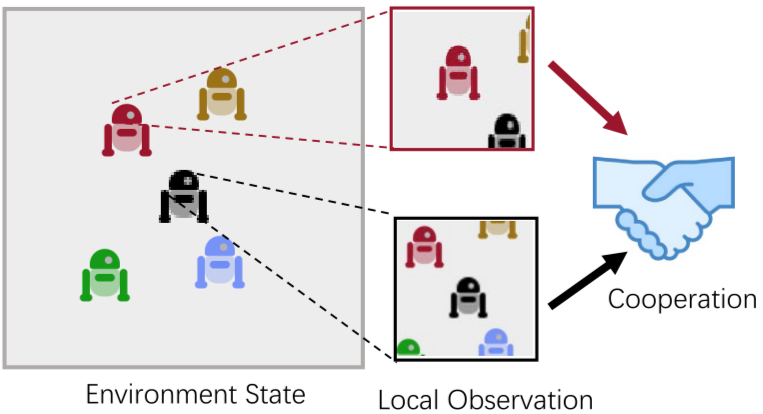
\includegraphics[width=0.8\linewidth]{Figures/partial_observation.png}
    \captionsetup{justification=centering}
    \caption{Partially observable state space for local agents.\footcite{moonlightMARL}}
    \label{fig:partial-observability}
\end{figure}
\footnotetext[7]{Adapted from \cite{moonlightMARL}.}
\subsubsection*{Agent Actions}\leavevmode

At each timestep, agents choose from a discrete action set:
\begin{itemize}
    \item \textbf{Detect Vacancy/Occupancy:} Use sensors (e.g., ultrasonic, camera) to scan adjacent cells.
    \item \textbf{Broadcast Update:} Transmit new occupancy/vacancy findings to nearby agents.
    \item \textbf{Relay Message:} Forward information from others to expand knowledge range.
    \item \textbf{Query Neighbors:} Request occupancy data for specific cells when local knowledge is outdated.
\end{itemize}

\subsubsection*{Multi-Agent Reinforcement Learning (MARL)}\leavevmode

\vspace{0.5em}
The Parking Mesh problem naturally maps onto a Multi-Agent Reinforcement Learning (MARL) framework. Each equipped vehicle functions as an autonomous agent, responsible for sensing local parking availability and sharing that information. Since efficient parking management depends on collective knowledge rather than isolated behavior, a cooperative MARL setup is ideal. In this setting, agents are not in competition but instead support one another by enhancing local awareness—ultimately reducing search times, easing congestion, and cutting emissions.

This collaborative structure allows the network as a whole to outperform isolated decision-making by maximizing shared objectives, such as minimizing drivers' parking time and improving urban traffic flow. Furthermore, the underlying architecture of the Parking Mesh—vehicles as nodes connected via short-range Bluetooth communication—lends itself naturally to a Graph Neural Network (GNN) implementation. GNNs are well-suited for modeling such relational data, as they propagate observations through network connections and capture inter-agent dynamics. By representing vehicles as graph nodes and their communication links as edges, GNNs enable the system to learn coordinated parking strategies that fully exploit the spatial and communicative structure of the mesh network.
 
% Discussion
\subsection{Reward Function}

The reward definition for an agent in our system needs to avoid issues that come with a delayed or infrequent reward. This can cause the learning to have a low convergence ability. To avoid this, we propose auxiliary rewards needed for faster convergence, such as penalties for frequent repetition of routes or extra driving distance. This is especially important since we have a high degree of constraints in our problem with the legality of parking in specific areas and due to the nature of parking being in high demand in metropolitan areas. However, the formal version of it will have to be found through iterations in order to optimize the behaviour of our agents. As we are acquiring more data, we will also adapt and improve the reward function.

\section{Model Architecture and Setup}
\subsection{Model Selection and Definition}
Despite being grounded in IoT and proximity sensing, our system still operates under partial observability. Each agent (driver) must make decisions without access to a global view of the environment. This challenge demands efficient coordination mechanisms. Research shows that Graph Neural Network (GNN)-based communication and centralized critic methods significantly improve agent performance in cooperative MARL (Multi-Agent Reinforcement Learning) environments like traffic or parking optimization\footcite{article}.

These findings highlight the need for communication mechanisms in our implementation—whether for shared observations, intent signalling, or updates about false positives/negatives. Such mechanisms become essential for agents to reconcile partial, noisy observations into actionable collective knowledge.

Our architecture is based on the Soft Actor-Critic (SAC) algorithm within a Centralized Training with Decentralized Execution (CTDE) framework. The central critic has access to global mesh data during training, while each actor acts independently at inference time using local sensor and Bluetooth inputs. This hybrid approach provides both training robustness and deployment flexibility.

The actor network is modeled as a Multi-Layer Perceptron (MLP) with two hidden layers of 256 neurons each, using LeakyReLU activations and a Softmax output. This structure balances expressivity with computational simplicity. For the critic, we explore three options:
\begin{itemize}
    \item \textbf{MLP:} Efficient for small input sizes; fast and easy to implement.
    \item \textbf{GNN:} Scales across fleet sizes; enables message passing between nodes.
    \item \textbf{Graph + Attention Pooling (G+A):} Learns contextual factors like time-of-day or regional bias through attention mechanisms.
\end{itemize}
To improve generalization, we incorporate regularization techniques such as L1/L2 penalties and dropout.

\begin{figure}[H]
    \centering
    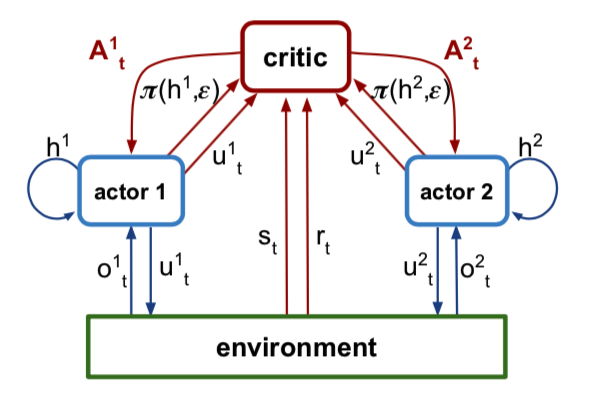
\includegraphics[width=0.8\linewidth]{Figures/c_critic.png}
    \captionsetup{justification=centering}
    \caption{Centralized critic architecture under CTDE.\footcite{Whiteson2020FactoredValue}}
    \label{fig:central-critic}
\end{figure}
\footnotetext[9]{Adapted from \cite{Whiteson2020FactoredValue}.}

To benchmark alternative MARL methods, we conducted a literature survey and compared several state-of-the-art algorithms\footcite{amato2024introductioncentralizedtrainingdecentralized} in terms of credit assignment, scalability, and applicability to a city-scale parking mesh\footcite{article}. The results are summarized below.

\begin{table}[htp]
\centering
\caption{COMA (Counterfactual MA-AC)}
\small
\begin{tabularx}{\linewidth}{>{\bfseries}p{3.5cm} >{\RaggedRight\arraybackslash}X}
\toprule
Credit Assignment & Per-agent counterfactual baseline \\
Strengths & Low-variance gradients on \textit{small} teams \\
Weaknesses & Critic input grows with $N$; unworkable when thousands of agents share a road graph \\
\bottomrule
\end{tabularx}
\end{table}

\FloatBarrier

\begin{table}[htp]
\centering
\caption{QMIX / VDN}
\small
\begin{tabularx}{\linewidth}{>{\bfseries}p{3.5cm} >{\RaggedRight\arraybackslash}X}
\toprule
Credit Assignment & Monotonic mixing of per-agent Q-values \\
Strengths & Scales to hundreds of agents \\
Weaknesses & Monotonic constraint fails under non-linear interactions (e.g., two cars blocking one lane) \\
\bottomrule
\end{tabularx}
\end{table}

\FloatBarrier

\begin{table}[htp]
\centering
\caption{MADDPG / MA-SAC}
\small
\begin{tabularx}{\linewidth}{>{\bfseries}p{3.5cm} >{\RaggedRight\arraybackslash}X}
\toprule
Credit Assignment & Central critic over joint observations \\
Strengths & Handles continuous control; replay-buffer friendly \\
Weaknesses & Critic overfits when $N > 50$; loses locality information \\
\bottomrule
\end{tabularx}
\end{table}

\FloatBarrier

\begin{table}[H]
\centering
\caption{MAGAC (Multi-Agent Graph Soft Actor Critic)}
\small
\begin{tabularx}{\linewidth}{>{\bfseries}p{3.5cm} >{\RaggedRight\arraybackslash}X}
\toprule
Credit Assignment & GNN critic with “soft” counterfactuals \\
Strengths & Near-linear scaling; exploits road topology; variable team sizes \\
Weaknesses & Requires neighbor graph and message-passing layers \\
\bottomrule
\end{tabularx}
\end{table}


Based on the above analysis, while COMA and QMIX have proven value in constrained team settings, they fail to scale to large agent populations or complex topologies. MAGAC emerges as the most promising candidate for our scenario, combining scalability, robustness, and architectural alignment with our graph-based parking mesh.

\subsubsection*{Soft Actor-Critic GNN Component}

Graph Neural Networks (GNNs) generalize convolution to problems whose natural structure is a graph—a set of nodes (vehicles) linked by edges (Bluetooth connections). Instead of sliding a fixed-size kernel across pixels, a GNN lets every node exchange “messages” with its neighbors, aggregate what it hears, and update its own hidden state. By stacking multiple message-passing layers, information propagates hop-by-hop—enabling each vehicle to reason not only about the parking bays it sees but also about availability cues relayed from cars two or three streets away.

At each message-passing step, every sender node \( j \) transforms its current embedding \( h_j^{(\ell - 1)} \) using a learned weight matrix \( W \) (or a small MLP). This transformed vector is concatenated with the receiver’s embedding \( h_i^{(\ell - 1)} \), and the pair is passed through an activation function such as \(\text{LeakyReLU}\) to produce a raw compatibility score \( e_{ij} \):

\[
e_{ij} = \text{LeakyReLU}(W[h_i^{(\ell - 1)} \Vert h_j^{(\ell - 1)}])
\]

The scores \( e_{ij} \) for all neighbors of node \( i \) are normalized using a softmax to yield attention coefficients \( \alpha_{ij} \):

\[
\alpha_{ij} = \frac{\exp(e_{ij})}{\sum_{k \in \mathcal{N}(i)} \exp(e_{ik})}
\]

These coefficients act as an adaptive attention kernel: for instance, a car that recently confirmed a vacancy may receive a high weight, while a distant or outdated neighbor receives little influence.

The reason GNNs are well-suited to our Parking Mesh system is scalability. The same shared weight matrix \( W \) operates whether there are 50 or 50{,}000 cars in the graph. Unlike an MLP critic that flattens the environment into a fixed-size vector, a GNN respects the road network’s structure, focusing computation on meaningful local interactions. This results in \textbf{linear scalability} with the number of edges—an essential feature for a real-time urban system.

\subsubsection*{Target-Network Implementation}

To mitigate the moving-target problem in off-policy learning, we maintain a separate \textbf{target critic network}—a periodically updated copy of the main GNN-based critic—that provides stable Q-value estimates during training. After each critic update, we softly update the target network parameters using \textbf{Polyak averaging}:

\[
\theta_{\text{target}} \leftarrow (1 - \tau)\,\theta_{\text{target}} + \tau\,\theta_{\text{critic}}
\]

where \( \tau = 0.005 \) is the update rate.

Rather than applying this update at every gradient step, we accumulate critic gradients over three mini-batches before performing both the optimizer step and the Polyak update. This staggered update reduces jitter in the target values and improves training stability.

The target network is initialized as an exact copy of the main critic at the start of training and then gradually tracks it through these soft updates. When computing Bellman backups during training, we use \textbf{clipped double Q-learning}—taking the minimum of the two target critic heads—to reduce overestimation bias:

\[
Q_{\text{target}} = \min\big(Q_{\text{target}}^{(1)},\, Q_{\text{target}}^{(2)}\big)
\]

This clipped estimate helps ensure that our centralized critic provides a \textbf{stable and conservative learning signal} for the decentralized actor policies, which is crucial for convergence in multi-agent systems like Parking Mesh.

​

% Conclusion
\subsection{Training Paradigm}

Centralised Training, Decentralised Execution (CTDE) is a widely used paradigm in Multi-Agent Reinforcement Learning (MARL), addressing coordination challenges among multiple autonomous agents. In this framework, agents are trained with access to \textbf{global state information}, allowing a centralised critic to evaluate joint actions and their overall impact. This shared view enables more stable learning, more accurate credit assignment, and improved coordination during training.

During execution, however, each agent operates independently using only its \textbf{local observations}—without global awareness or centralised control. This design ensures \textbf{scalability}, since adding more agents does not increase reliance on central infrastructure and helps avoid bottlenecks or single points of failure.

\begin{figure}[H]
    \centering
    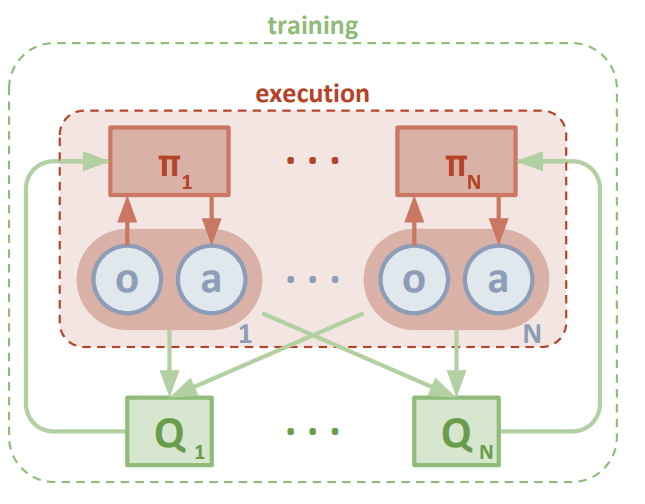
\includegraphics[width=0.7\linewidth]{Figures/CTDE.png}
    \caption{Centralised Training and Decentralised Execution (CTDE) framework.\footcite{lowe2017multiagent}}
    \label{fig:ctde-diagram}
\end{figure}
\footnotetext{Adapted from \cite{lowe2017multiagent}.}

CTDE excels in \textbf{partially observable environments}, where agents cannot fully perceive the environment on their own. Global training data helps agents learn to \textbf{infer hidden information} and develop \textbf{cooperative strategies}, even when each agent sees only a local slice of the world at execution time.

\vspace{0.5em}
\noindent\textbf{MAGAC in the CTDE Framework}

MAGAC aligns naturally with the CTDE paradigm and is highly suitable for the Parking Mesh system. During training, MAGAC employs a \textbf{centralised graph-based critic}, which aggregates observations and actions from all vehicles in the mesh. This enables the critic to model inter-agent dependencies—such as how one vehicle’s detection or relay of a vacancy affects others downstream.

At execution time, MAGAC uses \textbf{decentralised policies}: each vehicle computes its own actions based on \textbf{local sensor data and short-range Bluetooth messages} from neighbouring vehicles. This decentralised execution ensures the Parking Mesh is both scalable and robust—well-suited for dynamic urban environments.

By leveraging global information during training, MAGAC learns strategies that overcome the inherent \textbf{information asymmetry} in real-world parking. It enables vehicles to anticipate and propagate parking availability efficiently, even with limited visibility.

In summary, CTDE offers the ideal balance of central coordination during learning and distributed autonomy during real-world operation. MAGAC’s integration of centralised GNN-based training with decentralised, scalable execution makes it a natural fit for realising the vision of Parking Mesh: a city-wide, cooperative vehicle network that is low-cost, adaptive, and highly effective.

\subsection{Hyperparameters}
\subsubsection*{1. SAC Network Architecture and Optimization Setup}

Both actor and critic networks are trained using the \textbf{Adam optimizer} with standard parameters (\( \beta_1 = 0.9 \), \( \beta_2 = 0.999 \), \( \epsilon = 1 \times 10^{-8} \)), ensuring robust convergence even under the non-stationarity induced by simultaneously learning agents—each representing a vehicle acting in the environment. 

We set the discount factor \( \gamma = 0.99 \) to balance short-term incentives (e.g., immediately reporting nearby parking spots) with longer-term cooperative benefits (such as improving downstream coverage for other drivers). 

Actor and critic learning rates are initially set to \( 3 \times 10^{-4} \), though we often accelerate the critic to \( 6 \times 10^{-4} \) to improve value convergence. \textbf{Gradient clipping} at a global norm of 0.8 prevents training spikes caused by rare but impactful transitions, such as sudden multi-spot vacancies. 

Finally, we apply \textbf{cosine annealing schedules} to both learning rates, gradually reducing them over time to stabilize late-stage policy refinement.

\vspace{1em}

\subsubsection*{2. Automatic Entropy Tuning in SAC}

To maintain effective exploration during training, we employ \textbf{automatic entropy temperature tuning} for the actor policy. In the Soft Actor-Critic (SAC) framework, the policy seeks to maximize both expected return and entropy. The objective becomes:

\[
J_\pi = \mathbb{E}_{(s, a) \sim \pi} \left[ Q(s, a) - \alpha \log \pi(a|s) \right]
\]

Here, \( \alpha \) is the entropy temperature, which controls the trade-off between exploitation and exploration. Rather than fixing \( \alpha \), we adaptively tune it during training to match a target policy entropy \( \mathcal{H}_{\text{target}} \). For discrete action spaces, we follow the convention:

\[
\mathcal{H}_{\text{target}} = -\log |A_i|
\]

where \( |A_i| \) is the number of discrete actions available to agent \( i \). This encourages early stochasticity and progressively sharper policies as learning progresses. The entropy target is optimized using a separate \textbf{Adam optimizer} (learning rate \( 3 \times 10^{-4} \)), adjusting \( \alpha \) to minimize the KL divergence between the actual and target entropy.

This mechanism is especially valuable in our multi-agent parking setting, where deterministic policies risk early convergence to suboptimal regions or information bottlenecks in the city grid.

\vspace{1em}

\subsubsection*{3. Graph Neural Network Hyperparameters}

To stabilize training across varying graph sizes, we apply \textbf{layer normalization} after each aggregation step and include \textbf{residual connections}. 

Edge features consist of relative GPS offsets (\( \Delta x, \Delta y \)) and link quality (RSSI), giving three additional dimensions to inform the GNN of both spatial geometry and communication reliability. We apply dropout with \( p = 0.1 \) on the second GNN layer to prevent overfitting to frequent traffic patterns.

All GNN weights are optimized with Adam (using the same configuration as MLPs) to allow smooth adaptation to the evolving mesh topology.

\vspace{1em}

\subsubsection*{4. Multi-Agent Training Hyperparameters}

During real-time deployment, the number of agents equals the number of active app users in Madrid—potentially tens of thousands—each executing only its local actor policy. 

For centralized training, we simulate a representative subset (e.g., 500–1,000 agents) to remain within GPU constraints, rotating through random city sectors to expose the network to varied traffic densities.

Rollouts are fully off-policy with a rollout length of 1, enabling continual collection of transitions without resets—matching the always-on nature of parking dynamics. The critic is updated every environment step, while the actor is updated every two critic steps (1:2 ratio), ensuring policy changes are guided by accurate value estimates.

\textbf{Target network delays} of 3 updates are applied (Polyak updates occur only after three critic steps), reducing the variance in value targets. Gradients are clipped at a maximum norm of 0.8 to protect stability when abrupt state shifts occur, such as a sudden large-scale vacancy.

\vspace{1em}

\subsubsection*{5. Exploration and Entropy}

To balance exploitation of known parking hotspots with exploration of newly vacated areas, we rely on SAC’s \textbf{automatic entropy tuning}, targeting entropy \( \approx -|A_i| \) for a discrete action space of size around 10.

This dynamic \( \alpha \) tuning eliminates the need for hand-crafted exploration schedules across diverse zones—such as downtown vs. suburban regions.

We also optionally add \textbf{Gaussian action noise} with \( \sigma = 0.15 \) to the actor’s categorical logits prior to sampling. This smooths decision boundaries between similar actions (e.g., “broadcast cell (1,0)” vs. “broadcast cell (1,1)”), improving robustness and stochasticity across both dense and sparse regions of the environment.
                                          

\section{Data Pipeline}


The Parking Mesh system relies on a robust and scalable data pipeline to collect, process, and transform sensor and communication data into actionable learning signals and real-time driver guidance. This pipeline supports both the training of reinforcement learning agents and operational decision-making during live deployment.

\subsection{Data Sources}
Our system draws from three primary data sources. First, vehicle-based sensors such as proximity detectors identify adjacent parking vacancies. Optional enhancements like GPS, inertial measurement units, or cameras provide additional spatial and contextual information. Second, vehicles exchange real-time messages using Bluetooth mesh communication, reporting observed parking statuses and relaying received data. Third, simulated environments, particularly CityFlow and CARLA, generate synthetic traffic data across diverse urban conditions, supporting controlled, large-scale experimentation during model development.

\subsection{Ingestion and Preprocessing}
Raw data is ingested through several mechanisms. Edge aggregation modules running on each vehicle process sensor input, apply noise filtering, batch events, and assign timestamps before broadcasting. During centralized training, this data is uploaded to replay buffers via secure Wi-Fi or cellular connections. In parallel, all spatial inputs, such as GPS coordinates, are normalized and mapped to a grid-based city representation that aligns with the system’s reinforcement learning environment.

\subsection{Feature Extraction}
Each incoming data point is converted into a structured vector. This includes the binary or probabilistic occupancy status of a cell, metadata such as zoning type, time-of-day, and parking regulations, as well as the vehicle’s relative position and movement direction. Communication attributes such as message latency or Bluetooth signal strength are also embedded. These feature vectors are used both by actor-critic networks during training and by real-time inference modules during deployment.

\subsection{Labeling}
In simulation and pilot deployments, ground truth labels—such as confirmed successful parking or collisions—are generated to support auxiliary supervised losses and improved reward shaping. This feedback improves early-stage learning and helps agents converge more efficiently by reinforcing useful behaviors.

\subsection{Storage and Query Interface}
All processed data is stored in a structured format that supports rapid querying and batch training. We use file formats such as Parquet and TFRecords for compact storage. For similarity search and trajectory analysis, we employ vector databases, while time-series stores like InfluxDB track system-level performance over time.

\subsection{Feedback Loop for Online Learning}
During deployment, anonymized performance logs—such as parking success rates and rerouting frequencies—are funneled back into the training pipeline. This enables continual policy refinement through online learning, allowing Parking Mesh to remain responsive to changing urban dynamics and driver behaviors.


\section{Operationalization and Deployment}
\subsection{Implementation Frameworks and Toolchain}

To build the Parking Mesh system end-to-end, we begin entirely in software. A microscopic traffic simulator such as \textbf{CityFlow} lets us import the full Madrid road graph (via OpenStreetMap) and run hundreds of thousands of vehicles faster than real time, while exposing a Python API that integrates directly into a custom \texttt{ParkingMeshEnv}. When richer perception and sensor noise are needed, we can replay the same episodes inside \textbf{CARLA}, or if traffic-signal logic becomes a concern, replace CityFlow with \textbf{SUMO} using the \texttt{SUMO-RL} Gym wrapper. All three simulators support the standard \texttt{observation}/\texttt{step}/\texttt{reset} interface, keeping experimentation seamless.

On the learning side, we use \textbf{PettingZoo} to wrap the simulator in a standard multi-agent API and control it using \textbf{Ray RLlib}. RLlib includes scalable implementations of \textbf{Soft Actor-Critic}, centralised critic templates, replay buffers, and elastic rollout workers—so we only need to register our \texttt{MAGAC} model. This model is implemented in \textbf{PyTorch}, with the graph-attention critic built using just two calls to \texttt{torch\_geometric.nn.GATConv} from \textbf{PyTorch Geometric} (or equivalent layers in \textbf{DGL} if preferred). Because the message-passing layers operate on sparse adjacency matrices, the critic scales linearly with the number of Bluetooth edges—even when simulating four million grid cells.

Training at city scale requires multiple GPUs. A small \textbf{Ray cluster} orchestrated by \textbf{Docker Compose} spins up dozens of rollout workers, each responsible for simulating a different tile of Madrid. Docker—running with the \texttt{nvidia} runtime—ensures a reproducible software stack. Adding compute is as simple as:

\begin{quote}
\texttt{docker compose up --scale worker=32}
\end{quote}

If the critic eventually grows large enough to require multi-GPU synchronization, we can integrate \textbf{Horovod} from UBER to perform all-reduce gradient updates without changing the model code.

\vspace{1em}

\noindent\textbf{Implementation proceeds in three phases:}

\begin{enumerate}
    \item \textbf{Prototype:} Wrap CityFlow, implement the MAGAC model, and train until convergence on a one-square-kilometre patch using a single GPU.
    
    \item \textbf{Scale-out:} Distribute training across a Ray cluster, introduce curriculum learning from light to rush-hour demand, and demonstrate convergence across the entire Madrid road graph.
    
    \item \textbf{Hardware-in-the-loop:} Compile the trained actor to \texttt{ONNX} and deploy to a two-district pilot with several hundred real vehicles. The same toolchain supports nightly fine-tuning using live telemetry, enabling Parking Mesh to evolve from a research prototype into a continuously adapting, city-scale infrastructure layer.
\end{enumerate}

\subsection{MLOps}

The deployment model is based on a two-path parallel strategy that addresses both geographic expansion and partnership integration. The first strategy employs a phased city district roll-out, beginning with a small pilot in 1-2 high-demand areas with 100-200 sensor-equipped vehicles. This initial roll-out demonstrates the core value proposition while maintaining low infrastructure complexity. After positive validation, the expansion phase extends coverage to 5-10 additional districts, scaling to 1,000-2,000 vehicles and implementing the first model updates derived from real-world data. Concurrently, a partnership-led deployment strategy targets existing fleets—taxi, delivery fleets, car-sharing etc—to maximize coverage thanks to vehicles that already travel through dense urban areas.

The MLOps pipeline design employs a multi-stage approach optimized for distributed networks. Data collection begins at the vehicle level, where ultra-low-power proximity sensors detect close-by parking spaces with signals preprocessed by onboard micro controllers to eliminate noise and normalize formats (if possible). This edge computing approach significantly reduces transmission overhead. The data pipeline implements strict data anonymization regarding vehicle identifiers, such that the data sent from the vehicle is limited to location coordinates and timestamps only. Telemetry aggregates are stored in cloud storage by district and timestamp to enable both historical analysis and real-time serving. Automated quality assurance operations check for spatial consistency and detect anomalous patterns that may be indicative of sensor faults or tampering incidents. The training infrastructure utilizes containerized environments with Graph Neural Network (GNN) components specifically optimized for the spatial relationships inherent in parking networks Training runs are based on a double-trigger system—time-scheduled (weekly for pilot, monthly for expansion) and threshold-triggered when measures of performance indicate drift outside of acceptable parameters. The assessment process uses champion-challenger competitions where new models run in shadow mode, making decisions on real data but not influencing actions. Model deployment follows a canary release form, growing incrementally from one district to the entire network, with automatic rollback capability triggered by anomaly detection systems that monitor technical performance, as well as user-reported satisfaction measures. 

Regarding Cloud infrastructure deployment providers, we decided to architect the infrastructure using AWS, but alternatives such as Microsoft Azure are also viable. The AWS system relies on EC2 Spot Instances for cost-effective training, alongside reserved instances for stable inference, with data flowing through a data lake in S3 with partitioned buckets (raw, processed, models) and real-time availability served by DynamoDB. Containerized microservices executed by ECS/Fargate manage the model life cycle from training to evaluation and phased deployment, while SageMaker components offer version control, automated workflow, explainability and drift detection. Azure also facilitates these through AKS, IoT Hub, Blob Storage, Cosmos DB and Azure ML, albeit with enterprise benefits for city-level deployments.
\begin{figure}[H]
    \centering
    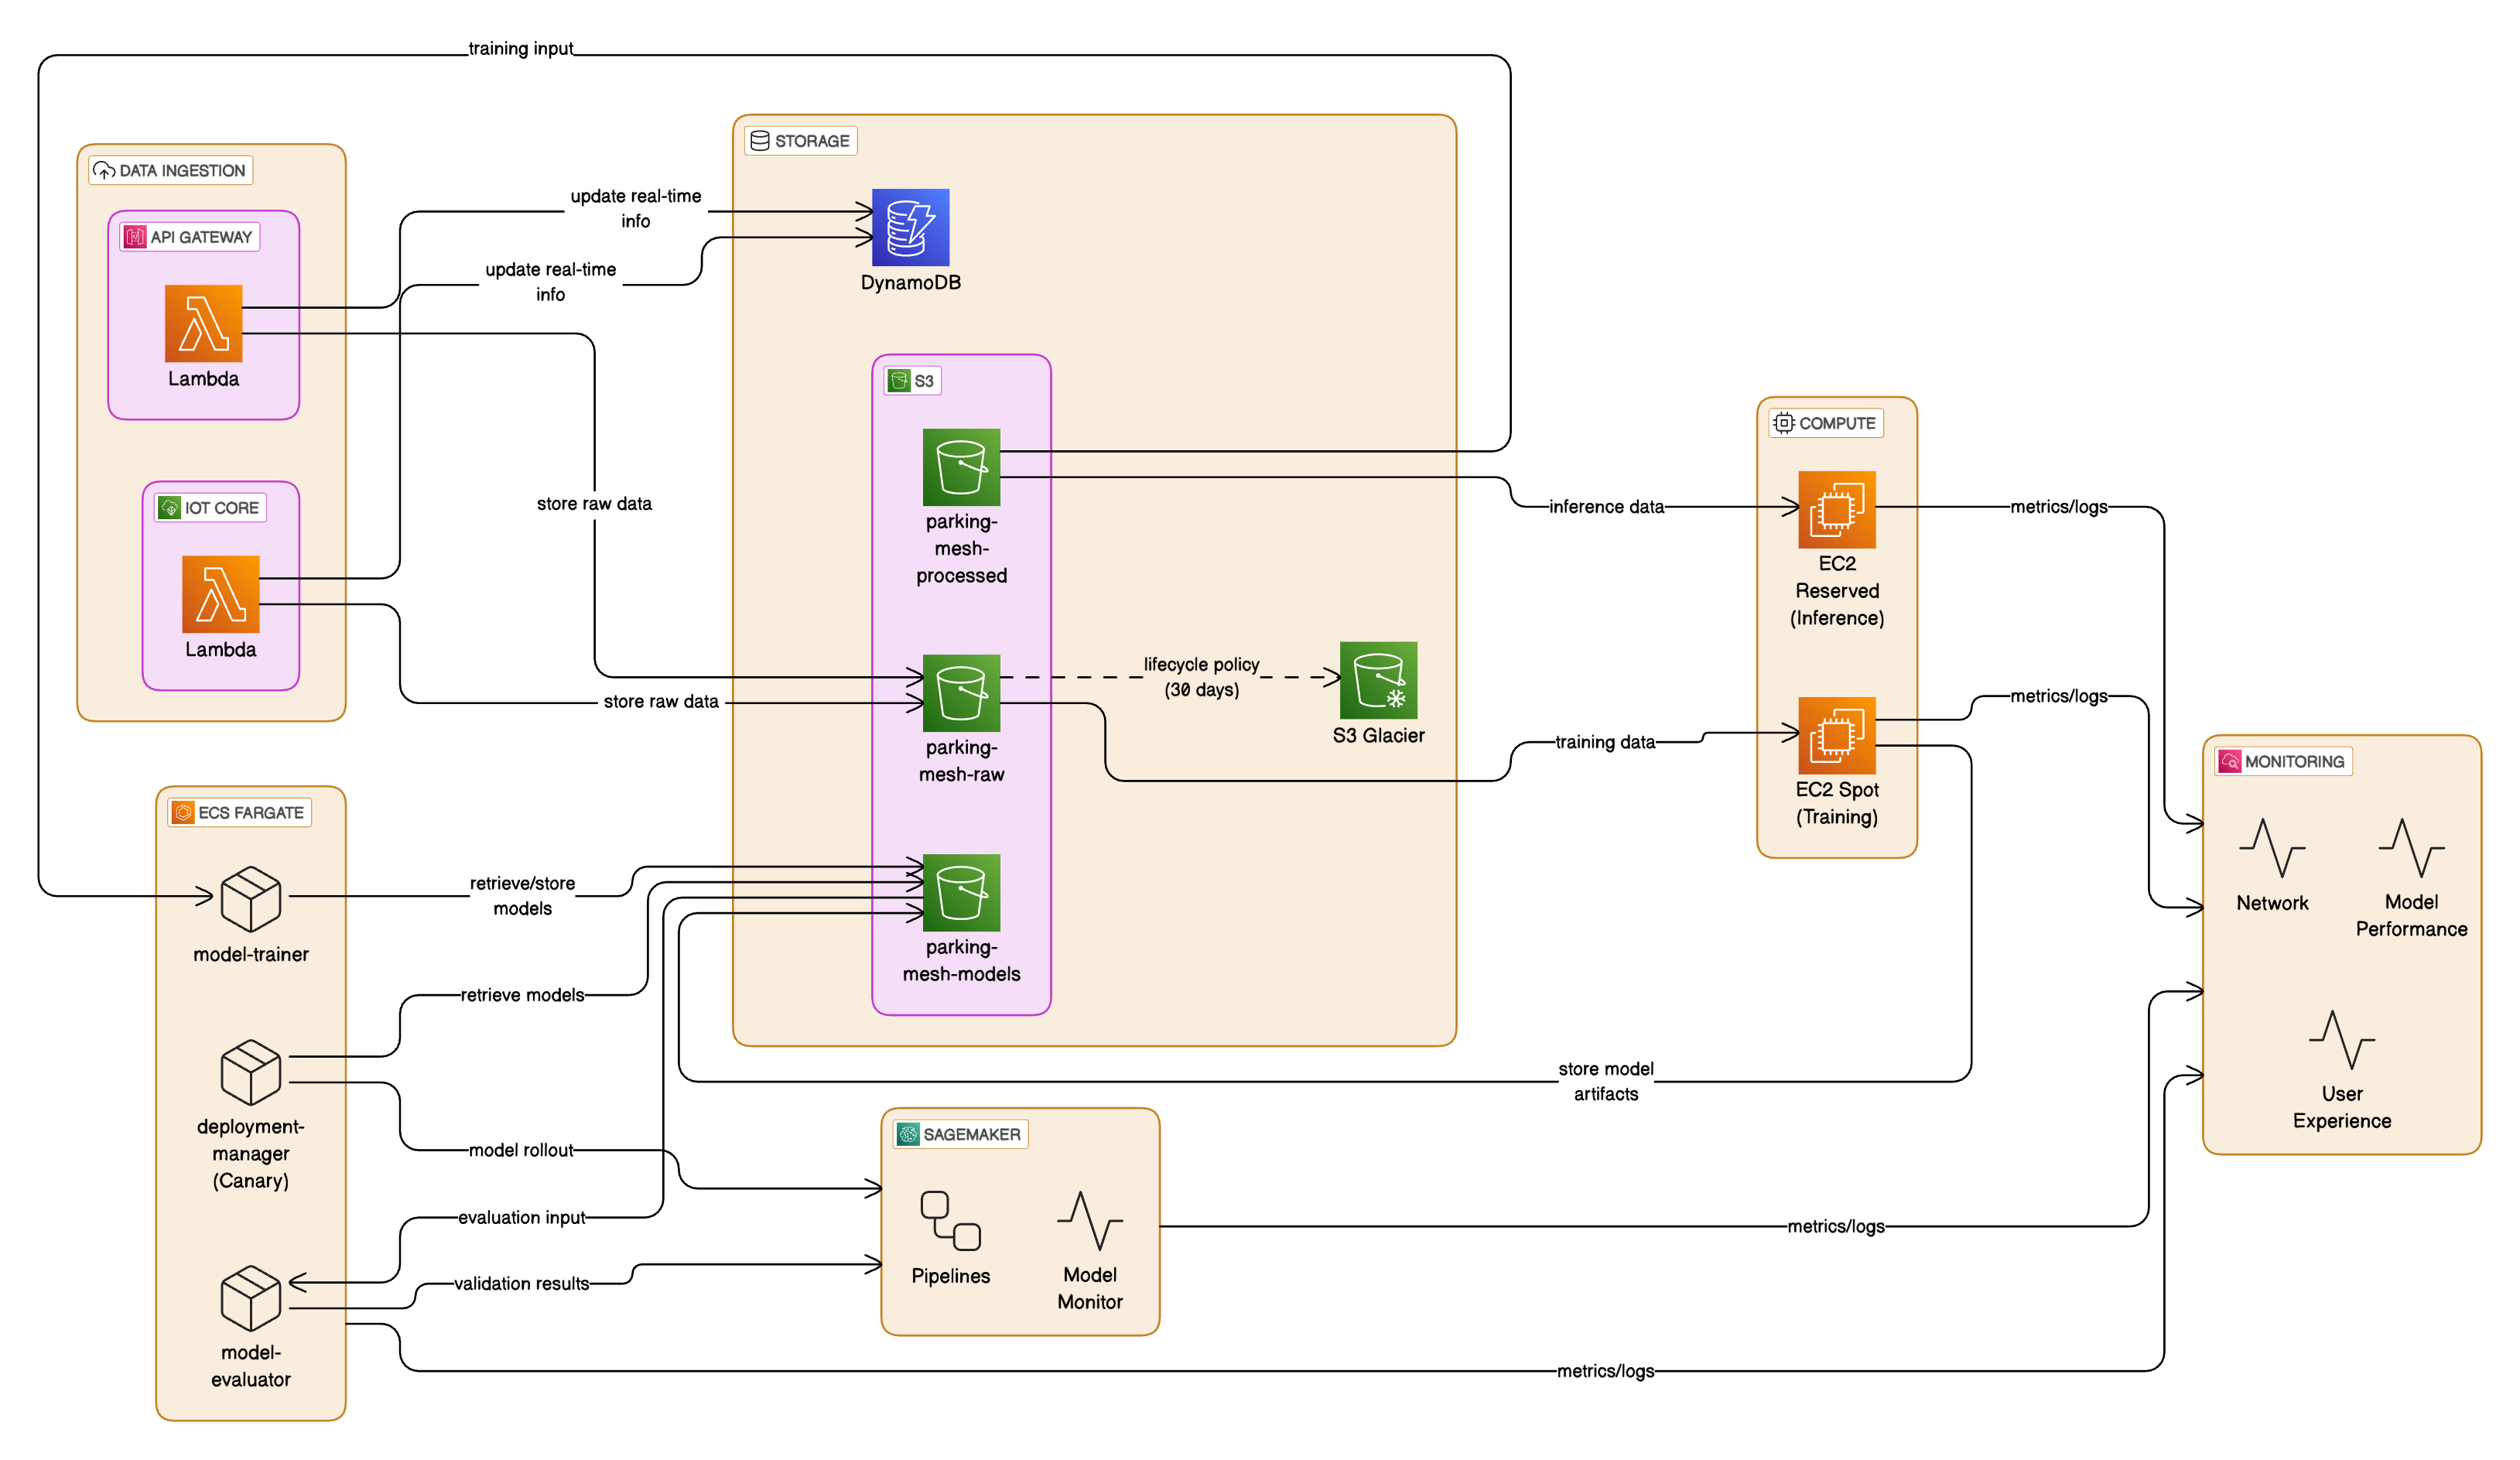
\includegraphics[width=\linewidth]{Figures/mlops.png} % increased from 0.8 to 1.0
    \captionsetup{justification=centering}
    \caption{Diagram of cloud infrastructure.}
    \label{fig:Deployment}
\end{figure}
\subsection{Risk Mitigation Measures}

Several risks have been identified in the system. Sensor faults and failures could undermine data quality, which will be addressed through periodic calibration procedures. Privacy concerns arising from location data collection will be mitigated through encryption and privacy-by-design protocols. Mesh network vulnerabilities, such as false or malicious vacancy reports, will be countered using trust scoring and anomaly detection systems that monitor and validate node behaviors within the network.
\subsection{Virtuous Data Cycle}

To maintain performance over time, agent policies will be retrained quarterly using anonymized, aggregated performance data collected by the system. This process allows the system to adapt dynamically to changes in city layouts, traffic patterns, and parking behavior. Future development may include integration of federated learning approaches, enabling neighborhoods or districts to locally refine policies without central data aggregation, preserving privacy while enhancing performance and avoiding model drift.

\section{Future Development}


Looking ahead, the Parking Mesh system presents numerous opportunities for advancement across hardware, software, and deployment dimensions. These developments aim to enhance real-world effectiveness, support broader adoption, and elevate the overall impact on urban mobility.

\subsection{Edge Hardware Evolution}

We plan to evolve our sensing hardware by integrating additional sensor modalities such as low-cost cameras, GPS-IMUs, or radar for more accurate spatial mapping. Incorporating real-time sensor fusion on edge devices will enable improved detection of dynamic changes like double-parking or temporary construction. Additionally, migrating from basic microcontrollers to edge AI chips (e.g., NVIDIA Jetson Nano or Google Coral) will enable in-situ inference and local decision-making without reliance on centralized cloud infrastructure.

\subsection{Adaptive Reward Tuning}

Future versions of the reinforcement learning component will adopt meta-learning techniques to dynamically adjust reward functions based on traffic density, user behavior, and parking demand fluctuations. This will ensure robust agent behavior in evolving urban conditions and allow agents to generalize across cities without extensive retraining. Moreover, we envision integrating personalized agent objectives based on user preferences (e.g., proximity to entrance, price sensitivity) through multi-objective RL.

\subsection{Federated Learning Deployment}

To preserve data privacy and reduce transmission overhead, we aim to implement federated learning. This will allow local vehicle policies to be trained on-device and periodically synced via encrypted updates, enabling continuous learning while safeguarding user data. Such a model is particularly suited to a privacy-sensitive application like parking, where location data is inherently personal.

\subsection{Interoperability with Smart Infrastructure}

Our roadmap includes integration with existing and emerging smart city infrastructure such as traffic signals, toll systems, and municipal IoT networks. Bidirectional communication with these systems can provide additional contextual data (e.g., event-based congestion, road closures) and enable coordinated city-wide optimizations beyond parking.

\subsection{Real-World Pilot Scaling}

Following initial two-district pilots, we intend to expand into larger urban zones with varying topology, socioeconomic demographics, and vehicle types. This scaling will test the robustness of our system under heterogeneous conditions. Longitudinal studies will assess environmental impact, user behavior shifts, and economic outcomes, generating policy-relevant insights for municipalities.

\section*{Acknowledgements}
This research project received support during the Reinforcement Learning course, instructed by Professor José Manuel Rey Gonzalez, teacher at the School of Science and Technology of IE University.

\section{Bibliography}
\printbibliography

\end{document}